% Options for packages loaded elsewhere
\PassOptionsToPackage{unicode}{hyperref}
\PassOptionsToPackage{hyphens}{url}
%
\documentclass[
]{article}
\usepackage{lmodern}
\usepackage{amssymb,amsmath}
\usepackage{ifxetex,ifluatex}
\ifnum 0\ifxetex 1\fi\ifluatex 1\fi=0 % if pdftex
  \usepackage[T1]{fontenc}
  \usepackage[utf8]{inputenc}
  \usepackage{textcomp} % provide euro and other symbols
\else % if luatex or xetex
  \usepackage{unicode-math}
  \defaultfontfeatures{Scale=MatchLowercase}
  \defaultfontfeatures[\rmfamily]{Ligatures=TeX,Scale=1}
\fi
% Use upquote if available, for straight quotes in verbatim environments
\IfFileExists{upquote.sty}{\usepackage{upquote}}{}
\IfFileExists{microtype.sty}{% use microtype if available
  \usepackage[]{microtype}
  \UseMicrotypeSet[protrusion]{basicmath} % disable protrusion for tt fonts
}{}
\makeatletter
\@ifundefined{KOMAClassName}{% if non-KOMA class
  \IfFileExists{parskip.sty}{%
    \usepackage{parskip}
  }{% else
    \setlength{\parindent}{0pt}
    \setlength{\parskip}{6pt plus 2pt minus 1pt}}
}{% if KOMA class
  \KOMAoptions{parskip=half}}
\makeatother
\usepackage{xcolor}
\IfFileExists{xurl.sty}{\usepackage{xurl}}{} % add URL line breaks if available
\IfFileExists{bookmark.sty}{\usepackage{bookmark}}{\usepackage{hyperref}}
\hypersetup{
  pdftitle={Building Deep Learning Models},
  pdfauthor={Peter R. Rijnbeek, Seng Chan You, Xiaoyong Pan, Jenna Reps},
  hidelinks,
  pdfcreator={LaTeX via pandoc}}
\urlstyle{same} % disable monospaced font for URLs
\usepackage[margin=1in]{geometry}
\usepackage{color}
\usepackage{fancyvrb}
\newcommand{\VerbBar}{|}
\newcommand{\VERB}{\Verb[commandchars=\\\{\}]}
\DefineVerbatimEnvironment{Highlighting}{Verbatim}{commandchars=\\\{\}}
% Add ',fontsize=\small' for more characters per line
\usepackage{framed}
\definecolor{shadecolor}{RGB}{248,248,248}
\newenvironment{Shaded}{\begin{snugshade}}{\end{snugshade}}
\newcommand{\AlertTok}[1]{\textcolor[rgb]{0.94,0.16,0.16}{#1}}
\newcommand{\AnnotationTok}[1]{\textcolor[rgb]{0.56,0.35,0.01}{\textbf{\textit{#1}}}}
\newcommand{\AttributeTok}[1]{\textcolor[rgb]{0.77,0.63,0.00}{#1}}
\newcommand{\BaseNTok}[1]{\textcolor[rgb]{0.00,0.00,0.81}{#1}}
\newcommand{\BuiltInTok}[1]{#1}
\newcommand{\CharTok}[1]{\textcolor[rgb]{0.31,0.60,0.02}{#1}}
\newcommand{\CommentTok}[1]{\textcolor[rgb]{0.56,0.35,0.01}{\textit{#1}}}
\newcommand{\CommentVarTok}[1]{\textcolor[rgb]{0.56,0.35,0.01}{\textbf{\textit{#1}}}}
\newcommand{\ConstantTok}[1]{\textcolor[rgb]{0.00,0.00,0.00}{#1}}
\newcommand{\ControlFlowTok}[1]{\textcolor[rgb]{0.13,0.29,0.53}{\textbf{#1}}}
\newcommand{\DataTypeTok}[1]{\textcolor[rgb]{0.13,0.29,0.53}{#1}}
\newcommand{\DecValTok}[1]{\textcolor[rgb]{0.00,0.00,0.81}{#1}}
\newcommand{\DocumentationTok}[1]{\textcolor[rgb]{0.56,0.35,0.01}{\textbf{\textit{#1}}}}
\newcommand{\ErrorTok}[1]{\textcolor[rgb]{0.64,0.00,0.00}{\textbf{#1}}}
\newcommand{\ExtensionTok}[1]{#1}
\newcommand{\FloatTok}[1]{\textcolor[rgb]{0.00,0.00,0.81}{#1}}
\newcommand{\FunctionTok}[1]{\textcolor[rgb]{0.00,0.00,0.00}{#1}}
\newcommand{\ImportTok}[1]{#1}
\newcommand{\InformationTok}[1]{\textcolor[rgb]{0.56,0.35,0.01}{\textbf{\textit{#1}}}}
\newcommand{\KeywordTok}[1]{\textcolor[rgb]{0.13,0.29,0.53}{\textbf{#1}}}
\newcommand{\NormalTok}[1]{#1}
\newcommand{\OperatorTok}[1]{\textcolor[rgb]{0.81,0.36,0.00}{\textbf{#1}}}
\newcommand{\OtherTok}[1]{\textcolor[rgb]{0.56,0.35,0.01}{#1}}
\newcommand{\PreprocessorTok}[1]{\textcolor[rgb]{0.56,0.35,0.01}{\textit{#1}}}
\newcommand{\RegionMarkerTok}[1]{#1}
\newcommand{\SpecialCharTok}[1]{\textcolor[rgb]{0.00,0.00,0.00}{#1}}
\newcommand{\SpecialStringTok}[1]{\textcolor[rgb]{0.31,0.60,0.02}{#1}}
\newcommand{\StringTok}[1]{\textcolor[rgb]{0.31,0.60,0.02}{#1}}
\newcommand{\VariableTok}[1]{\textcolor[rgb]{0.00,0.00,0.00}{#1}}
\newcommand{\VerbatimStringTok}[1]{\textcolor[rgb]{0.31,0.60,0.02}{#1}}
\newcommand{\WarningTok}[1]{\textcolor[rgb]{0.56,0.35,0.01}{\textbf{\textit{#1}}}}
\usepackage{longtable,booktabs}
% Correct order of tables after \paragraph or \subparagraph
\usepackage{etoolbox}
\makeatletter
\patchcmd\longtable{\par}{\if@noskipsec\mbox{}\fi\par}{}{}
\makeatother
% Allow footnotes in longtable head/foot
\IfFileExists{footnotehyper.sty}{\usepackage{footnotehyper}}{\usepackage{footnote}}
\makesavenoteenv{longtable}
\usepackage{graphicx,grffile}
\makeatletter
\def\maxwidth{\ifdim\Gin@nat@width>\linewidth\linewidth\else\Gin@nat@width\fi}
\def\maxheight{\ifdim\Gin@nat@height>\textheight\textheight\else\Gin@nat@height\fi}
\makeatother
% Scale images if necessary, so that they will not overflow the page
% margins by default, and it is still possible to overwrite the defaults
% using explicit options in \includegraphics[width, height, ...]{}
\setkeys{Gin}{width=\maxwidth,height=\maxheight,keepaspectratio}
% Set default figure placement to htbp
\makeatletter
\def\fps@figure{htbp}
\makeatother
\setlength{\emergencystretch}{3em} % prevent overfull lines
\providecommand{\tightlist}{%
  \setlength{\itemsep}{0pt}\setlength{\parskip}{0pt}}
\setcounter{secnumdepth}{5}
\usepackage{fancyhdr}
\pagestyle{fancy}
\fancyhead{}
\fancyhead[CO,CE]{Building Deep Learning Models}
\fancyfoot[CO,CE]{PatientLevelPrediction Package Version 3.1.0}
\fancyfoot[LE,RO]{\thepage}
\renewcommand{\headrulewidth}{0.4pt}
\renewcommand{\footrulewidth}{0.4pt}

\title{Building Deep Learning Models}
\author{Peter R. Rijnbeek, Seng Chan You, Xiaoyong Pan, Jenna Reps}
\date{2020-06-03}

\begin{document}
\maketitle

{
\setcounter{tocdepth}{2}
\tableofcontents
}
\hypertarget{introduction}{%
\section{Introduction}\label{introduction}}

Electronic Health Records (EHR) data is high dimensional, heterogeneous,
and sparse, which makes predictive modelling a challenge. In the early
days, the machine learning community mainly focused on algorithm
development, currently there is a shift to more powerful feature
engineering. Deep Learning models are widely used to automatically learn
high-level feature representations from the data, and have achieved
remarkable results in image processing, speech recognition and
computational biology. Recently, interesting results have been shown
using EHRs, but more extensive research is needed to assess the power of
Deep Learning in this domain.

This vignette describes how you can use the Observational Health Data
Sciences and Informatics (OHDSI)
\href{http://github.com/OHDSI/PatientLevelPrediction}{\texttt{PatientLevelPrediction}}
package to build Deep Learning models. This vignette assumes you have
read and are comfortable with building patient level prediction models
as described in the
\href{https://github.com/OHDSI/PatientLevelPrediction/blob/master/inst/doc/BuildingPredictiveModels.pdf}{\texttt{BuildingPredictiveModels}
vignette}. Furthermore, this vignette assumes you are familiar with Deep
Learning methods.

\hypertarget{background}{%
\section{Background}\label{background}}

Deep Learning models are build by stacking an often large number of
neural network layers that perform feature engineering steps, e.g
embedding, and are collapsed in a final softmax layer (basically a
logistic regression layer). These algorithms need a lot of data to
converge to a good representation, but currently the sizes of the EHR
databases are growing fast which would make Deep Learning an interesting
approach to test within OHDSI's
\href{https://academic.oup.com/jamia/article/25/8/969/4989437}{Patient-Level
Prediction Framework}. The current implementation allows us to perform
research at scale on the value and limitations of Deep Learning using
EHR data. For relatively small Target and Outcome cohorts, Deep Learning
is most probably not the best choice.

Most current Deep Learning research is performed in python and we have
developed a pipeline to interact with python. Multiple Deep Learning
backends have been developed, e.g.~Tensorflow, PyTorch, Keras (recently
also available in R) etc. In the package we have implemented interaction
with Keras in R and PyTorch in Python but we invite the community to add
other backends.

Many network architectures have recently been proposed and we have
implemented a number of them, however, this list will grow in the near
future. It is important to understand that some of these architectures
require a 2D data matrix,
i.e.~\textbar patient\textbar x\textbar feature\textbar, and others use
a 3D data matrix
\textbar patient\textbar x\textbar feature\textbar x\textbar time\textbar.
The \href{www.github.com/ohdsi/FeatureExtraction}{FeatureExtraction
Package} has been extended to enable the extraction of both data formats
as will be described with examples below.

Note that training Deep Learning models is computationally intensive,
our implementation therefore supports both GPU and CPU. It will
automatically check whether there is GPU or not in your computer. A GPU
is highly recommended for Deep Learning!

\hypertarget{non-temporal-architectures}{%
\section{Non-Temporal Architectures}\label{non-temporal-architectures}}

We implemented the following non-temporal (2D data matrix) architectures
using PyTorch:

\begin{verbatim}
1) Logistics regression (LRTorch)
   A simple softmax layer with l2 regularization

2) Feed forward network (MLPTorch) 
   Supports multilayer perceptron (mlp_type = MLP) and 
   Self-Normalizing Neural Networks (mlp_type = SNN)
   Reference: https://arxiv.org/abs/1706.02515
\end{verbatim}

For the above two methods, we implemented support for a stacked
autoencoder and a variational autoencoder to reduce the feature
dimension as a first step. These autoencoders learn efficient data
encodings in an unsupervised manner by stacking multiple layers in a
neural network. Compared to the standard implementations of LR and MLP
these implementations can use the GPU power to speed up the gradient
descent approach in the back propagation to optimize the weights of the
classifier.

Table 1: Non-Temporal Deep Learning Models Hyper-Parameters

\begin{longtable}[]{@{}lll@{}}
\toprule
\begin{minipage}[b]{0.10\columnwidth}\raggedright
Name\strut
\end{minipage} & \begin{minipage}[b]{0.34\columnwidth}\raggedright
Description\strut
\end{minipage} & \begin{minipage}[b]{0.47\columnwidth}\raggedright
Hyper-parameters\strut
\end{minipage}\tabularnewline
\midrule
\endhead
\begin{minipage}[t]{0.10\columnwidth}\raggedright
LRTorch\strut
\end{minipage} & \begin{minipage}[t]{0.34\columnwidth}\raggedright
Logistic Regression Model\strut
\end{minipage} & \begin{minipage}[t]{0.47\columnwidth}\raggedright
w\_decay (l2 regularization), epochs (number of epochs), class\_weight
(0 = inverse ratio between number of positive and negative examples, -1
= focal loss (\url{https://arxiv.org/abs/1708.02002}), or other),
autoencoder (apply stacked autoencoder?, vae (apply variational
autoencoder)\strut
\end{minipage}\tabularnewline
\begin{minipage}[t]{0.10\columnwidth}\raggedright
MLPTorch\strut
\end{minipage} & \begin{minipage}[t]{0.34\columnwidth}\raggedright
Multi-Layer Perceptron Model\strut
\end{minipage} & \begin{minipage}[t]{0.47\columnwidth}\raggedright
mlp\_type (MLP = default, SNN = self-normalizing neural network), size
(number of hidden nodes), w\_decay (l2 regularization), epochs (number
of epochs), class\_weight(0 = inverse ratio between number of positive
and negative examples, -1 = focal loss, or other), autoencoder (apply
stacked autoencoder), vae (apply variational autoencoder?)\strut
\end{minipage}\tabularnewline
\bottomrule
\end{longtable}

\#\#Example The approach for logistic regression (LRTorch) and the
Multi-Layer Perceptron (MLPTorch) is identical. Here we will take
LRTorch as an example.

You need to generate a \texttt{population} and \texttt{plpData} object
as described in more detail in
\href{https://github.com/OHDSI/PatientLevelPrediction/blob/master/inst/doc/BuildingPredictiveModels.pdf}{\texttt{BuildingPredictiveModels}
vignette}.

Alternatively, you can make use of the data simulator. The following
code snippet creates a population of 12000 patients.

\begin{Shaded}
\begin{Highlighting}[]
\KeywordTok{set.seed}\NormalTok{(}\DecValTok{1234}\NormalTok{)}
\KeywordTok{data}\NormalTok{(plpDataSimulationProfile)}
\NormalTok{sampleSize <-}\StringTok{ }\DecValTok{12000}
\NormalTok{plpData <-}\StringTok{ }\KeywordTok{simulatePlpData}\NormalTok{(}
\NormalTok{  plpDataSimulationProfile,}
  \DataTypeTok{n =}\NormalTok{ sampleSize}
\NormalTok{)}

\NormalTok{population <-}\StringTok{ }\KeywordTok{createStudyPopulation}\NormalTok{(}
\NormalTok{  plpData,}
  \DataTypeTok{outcomeId =} \DecValTok{2}\NormalTok{,}
  \DataTypeTok{binary =} \OtherTok{TRUE}\NormalTok{,}
  \DataTypeTok{firstExposureOnly =} \OtherTok{FALSE}\NormalTok{,}
  \DataTypeTok{washoutPeriod =} \DecValTok{0}\NormalTok{,}
  \DataTypeTok{removeSubjectsWithPriorOutcome =} \OtherTok{FALSE}\NormalTok{,}
  \DataTypeTok{priorOutcomeLookback =} \DecValTok{99999}\NormalTok{,}
  \DataTypeTok{requireTimeAtRisk =} \OtherTok{FALSE}\NormalTok{,}
  \DataTypeTok{minTimeAtRisk =} \DecValTok{0}\NormalTok{,}
  \DataTypeTok{riskWindowStart =} \DecValTok{0}\NormalTok{,}
  \DataTypeTok{addExposureDaysToStart =} \OtherTok{FALSE}\NormalTok{,}
  \DataTypeTok{riskWindowEnd =} \DecValTok{365}\NormalTok{,}
  \DataTypeTok{addExposureDaysToEnd =} \OtherTok{FALSE}\NormalTok{,}
  \DataTypeTok{verbosity =} \StringTok{"INFO"}
\NormalTok{)}
\end{Highlighting}
\end{Shaded}

As an example we will build a LRTorch model. We could specify the
stacked autoencoder or the variational autoencoder to be used for
reducing the feature dimension as an initial layer, but for this example
we do not.

\begin{Shaded}
\begin{Highlighting}[]
\NormalTok{autoencoder <-}\StringTok{ }\OtherTok{FALSE}
\NormalTok{vae <-}\StringTok{ }\OtherTok{FALSE}
\end{Highlighting}
\end{Shaded}

We added a class\_weight for imbalanced data, the default value 0 is the
inverse ratio between negatives and positives,-1 applies focal loss.

\begin{Shaded}
\begin{Highlighting}[]
\NormalTok{class_weight <-}\StringTok{ }\DecValTok{0}
\end{Highlighting}
\end{Shaded}

\begin{Shaded}
\begin{Highlighting}[]
\CommentTok{# Specify the settings for Logistics regression model using Torch in Python}
\NormalTok{model <-}\StringTok{ }\KeywordTok{setLRTorch}\NormalTok{(}\DataTypeTok{autoencoder=}\NormalTok{autoencoder, }\DataTypeTok{vae=}\NormalTok{vae,  }\DataTypeTok{class_weight=}\NormalTok{class_weight)}
\end{Highlighting}
\end{Shaded}

No we define our modelling parameters.

\begin{Shaded}
\begin{Highlighting}[]
\NormalTok{testFraction <-}\StringTok{ }\FloatTok{0.2}
\NormalTok{testSplit <-}\StringTok{ 'person'}
\NormalTok{nfold <-}\StringTok{ }\DecValTok{3}
\NormalTok{splitSeed <-}\StringTok{ }\DecValTok{1000}
\end{Highlighting}
\end{Shaded}

And we train and internally validate the model.

\begin{Shaded}
\begin{Highlighting}[]
\NormalTok{results <-}\StringTok{ }\NormalTok{PatientLevelPrediction}\OperatorTok{::}\KeywordTok{runPlp}\NormalTok{(}\DataTypeTok{population =}\NormalTok{ population, }
                                          \DataTypeTok{plpData =}\NormalTok{ plpData, }
                                          \DataTypeTok{modelSettings =}\NormalTok{ model,}
                                          \DataTypeTok{testSplit=}\NormalTok{testSplit,}
                                          \DataTypeTok{testFraction=}\NormalTok{testFraction,}
                                          \DataTypeTok{nfold=}\NormalTok{nfold, }
                                          \DataTypeTok{splitSeed=}\NormalTok{splitSeed) }
\end{Highlighting}
\end{Shaded}

\hypertarget{temporal-architectures}{%
\section{Temporal Architectures}\label{temporal-architectures}}

Several architectures are implemented that can handle temporal data in
PyTorch and R Keras.

\hypertarget{pytorch-cnn}{%
\subsection{PyTorch CNN}\label{pytorch-cnn}}

We implemented the following \textbf{convolutional} models described in
\url{https://github.com/clinicalml/deepDiagnosis} in CNNTorch:

\begin{enumerate}
\def\labelenumi{\arabic{enumi})}
\item
  Temporal Convolutional neural network over a backward window (type =
  cnn)

  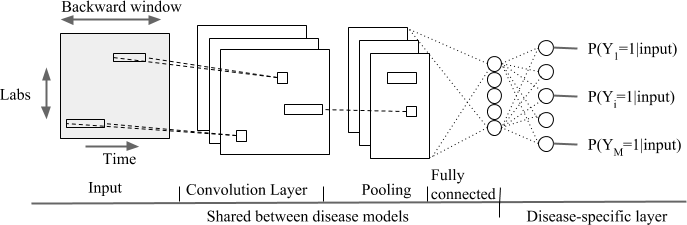
\includegraphics{arch1.png}
\item
  Convolutional neural network over input and time dimension (type =
  mix)

  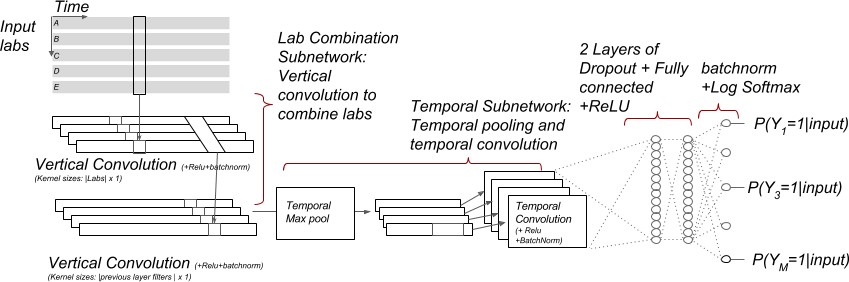
\includegraphics{conv_arch2.png}
\item
  Multi-resolution temporal convolutional neural network (type = multi)

  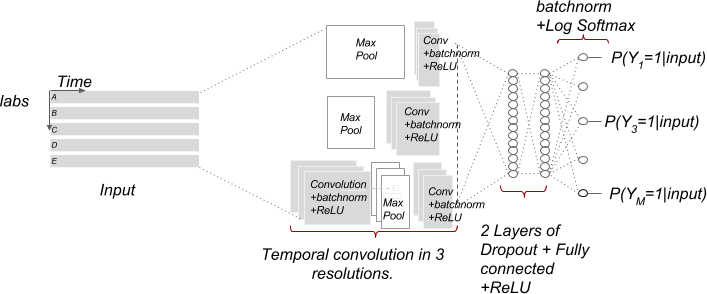
\includegraphics{conv_arch1.png}
\end{enumerate}

Furthermore, we added the following achitectures:

\begin{enumerate}
\def\labelenumi{\arabic{enumi})}
\setcounter{enumi}{3}
\item
  CNN with filters with three different parallel kernel sizes (3,4,5)
  and a fully connected layers (type = mlf)

  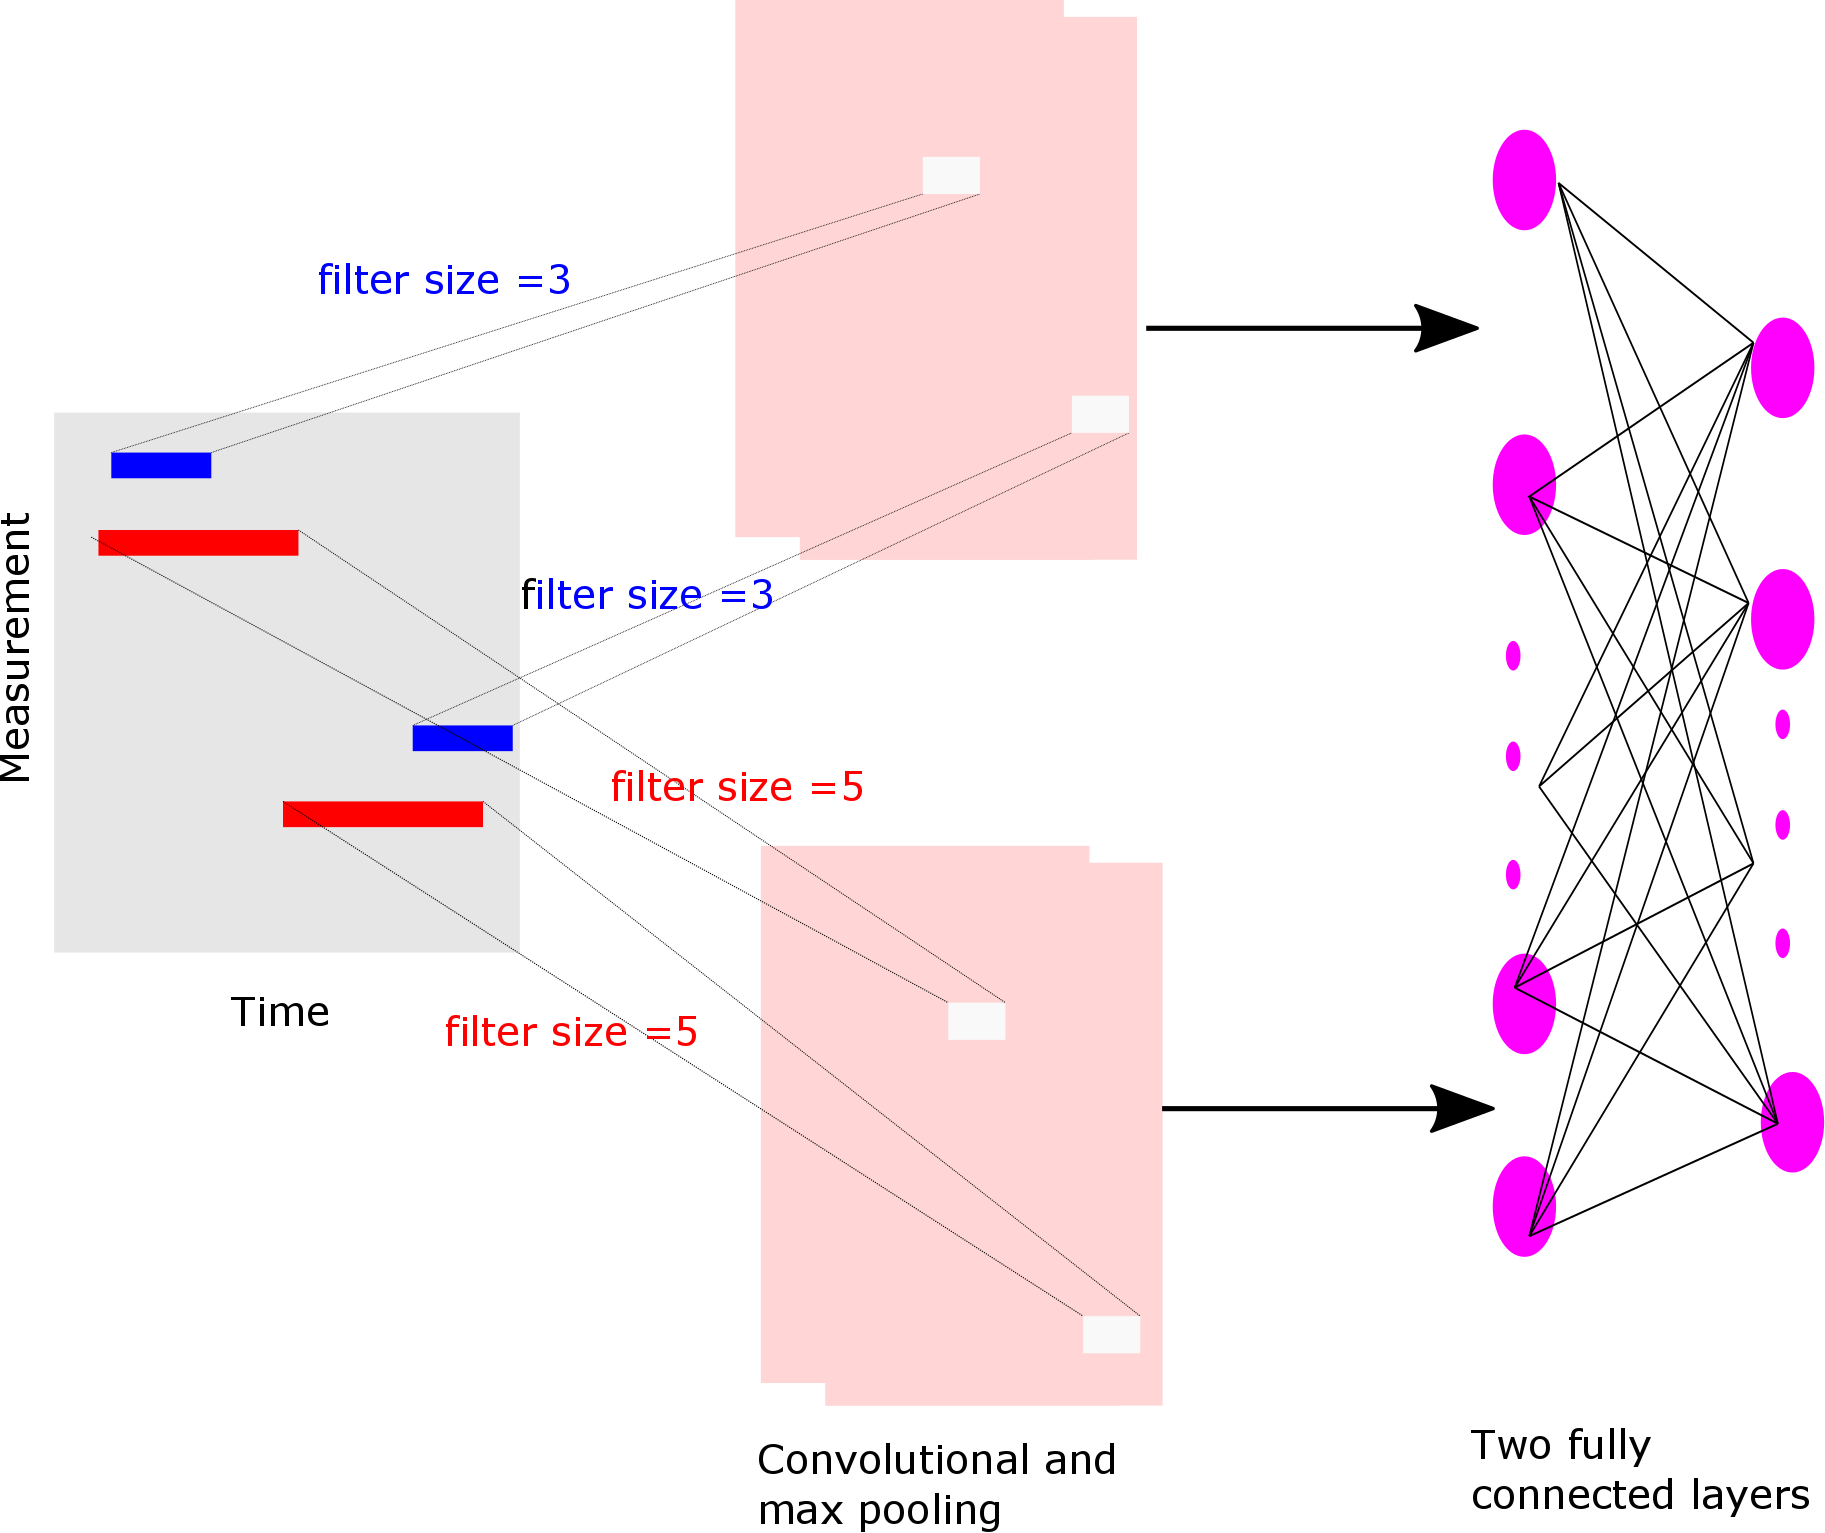
\includegraphics{cnn_mlf2.png}
\item
  LSTM network over the backward window (type = lstm)

  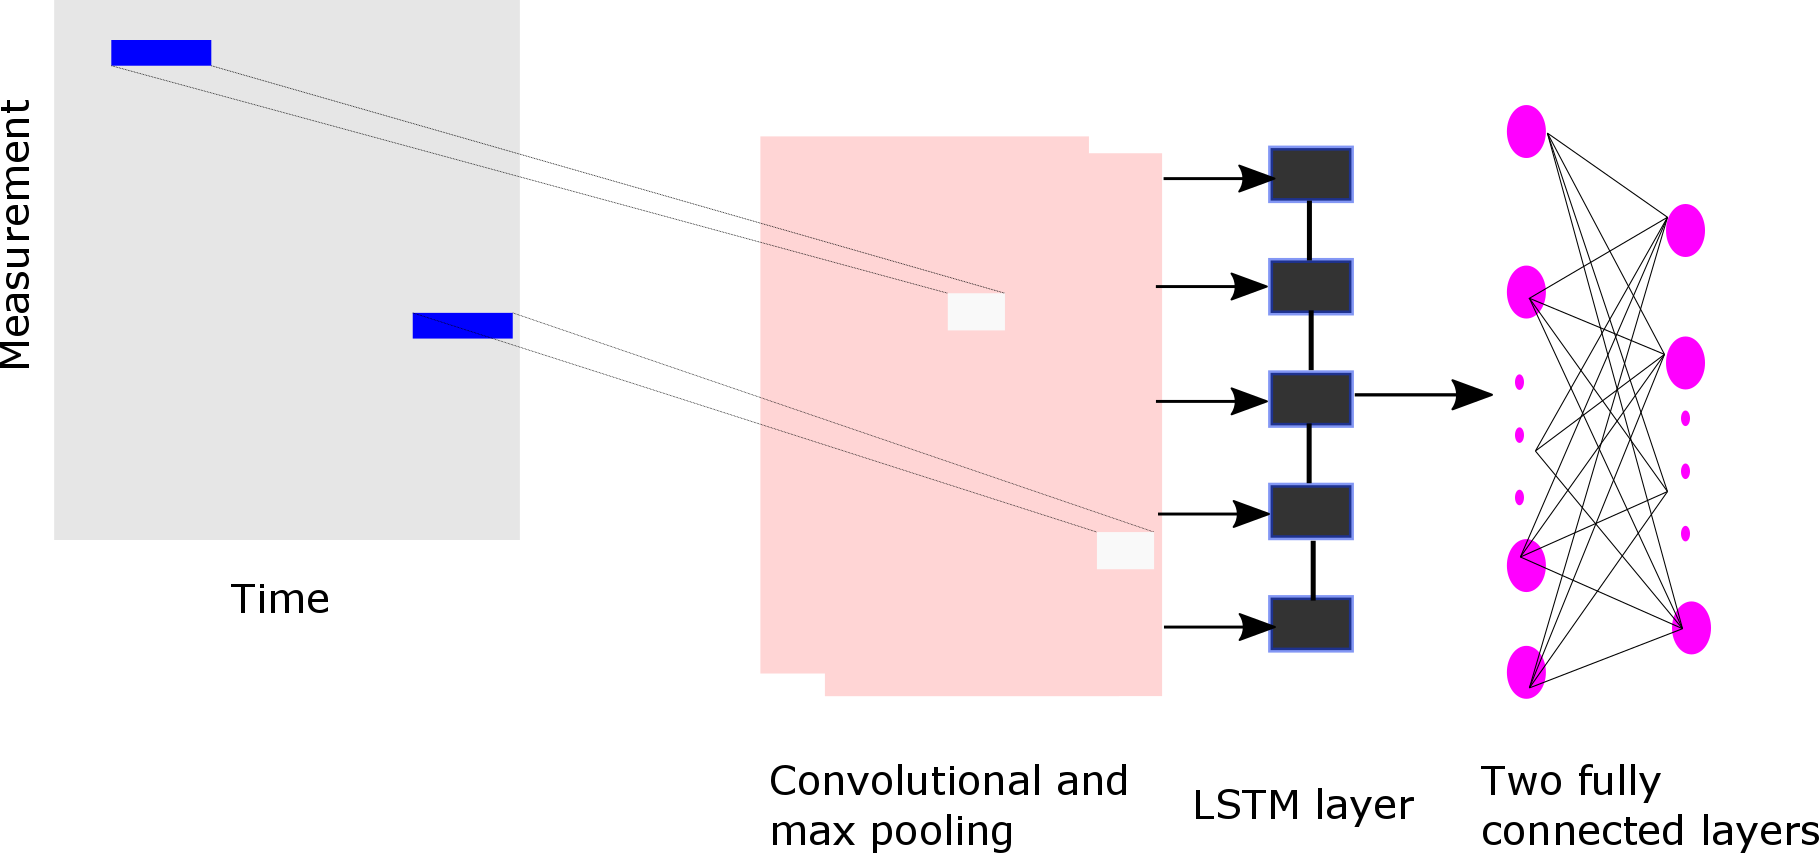
\includegraphics{cnn_lstm.png}
\item
  Residual Learning Network as described in:
  \url{https://arxiv.org/abs/1512.03385} (type = resnet)

  This a very big network, see the paper for the topology.
\end{enumerate}

\begin{longtable}[]{@{}ll@{}}
\toprule
\begin{minipage}[b]{0.26\columnwidth}\raggedright
parameter\strut
\end{minipage} & \begin{minipage}[b]{0.68\columnwidth}\raggedright
description\strut
\end{minipage}\tabularnewline
\midrule
\endhead
\begin{minipage}[t]{0.26\columnwidth}\raggedright
nbfilters\strut
\end{minipage} & \begin{minipage}[t]{0.68\columnwidth}\raggedright
The number of convolution filters\strut
\end{minipage}\tabularnewline
\begin{minipage}[t]{0.26\columnwidth}\raggedright
epochs\strut
\end{minipage} & \begin{minipage}[t]{0.68\columnwidth}\raggedright
The number of epochs\strut
\end{minipage}\tabularnewline
\begin{minipage}[t]{0.26\columnwidth}\raggedright
seed\strut
\end{minipage} & \begin{minipage}[t]{0.68\columnwidth}\raggedright
Random seed\strut
\end{minipage}\tabularnewline
\begin{minipage}[t]{0.26\columnwidth}\raggedright
class\_weight\strut
\end{minipage} & \begin{minipage}[t]{0.68\columnwidth}\raggedright
The class weight used for imbalanced data (0: Inverse ratio between
positives and negatives, -1: Focal loss, or number)\strut
\end{minipage}\tabularnewline
\bottomrule
\end{longtable}

\hypertarget{pytorch-rnn}{%
\subsection{PyTorch RNN}\label{pytorch-rnn}}

The following \textbf{recurrent neural network} models are implemented
in RNNTorch:

\begin{enumerate}
\def\labelenumi{\arabic{enumi})}
\item
  RNN with one LSTM layer fed into one fully connected layer (type =
  RNN)

  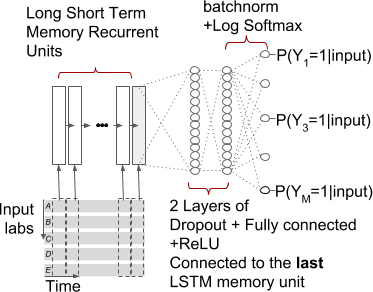
\includegraphics{lstm_last.png}
\item
  RNN with one bidirectional LSTM layer fed into one fully connected
  layer (type = BiRNN)

  This network looks the same as above but then as a bi-directional
  version
\item
  One Gated Recurrent Unit layer fed into one fully connected layers
  (type = GRU)

  This network looks the same as above but then implemented as GRU
\end{enumerate}

The following hyper-parameters can be set for these PyTorch models:

\begin{longtable}[]{@{}ll@{}}
\toprule
\begin{minipage}[b]{0.26\columnwidth}\raggedright
parameter\strut
\end{minipage} & \begin{minipage}[b]{0.68\columnwidth}\raggedright
description\strut
\end{minipage}\tabularnewline
\midrule
\endhead
\begin{minipage}[t]{0.26\columnwidth}\raggedright
hidden\_size\strut
\end{minipage} & \begin{minipage}[t]{0.68\columnwidth}\raggedright
The number of features in hidden state\strut
\end{minipage}\tabularnewline
\begin{minipage}[t]{0.26\columnwidth}\raggedright
epochs\strut
\end{minipage} & \begin{minipage}[t]{0.68\columnwidth}\raggedright
The number of epochs\strut
\end{minipage}\tabularnewline
\begin{minipage}[t]{0.26\columnwidth}\raggedright
seed\strut
\end{minipage} & \begin{minipage}[t]{0.68\columnwidth}\raggedright
Random seed\strut
\end{minipage}\tabularnewline
\begin{minipage}[t]{0.26\columnwidth}\raggedright
class\_weight\strut
\end{minipage} & \begin{minipage}[t]{0.68\columnwidth}\raggedright
The class weight used for imbalanced data (0: Inverse ratio between
positives and negatives, -1: Focal loss, or number)\strut
\end{minipage}\tabularnewline
\bottomrule
\end{longtable}

\newpage

\hypertarget{r-keras-cnn}{%
\subsection{R Keras CNN}\label{r-keras-cnn}}

The following temporal architectures as described in
\url{https://arxiv.org/pdf/1608.00647.pdf} were implemented using R
Keras:

\begin{enumerate}
\def\labelenumi{\arabic{enumi}.}
\item
  Multi-resolution CovNN model (CovNN.R)

  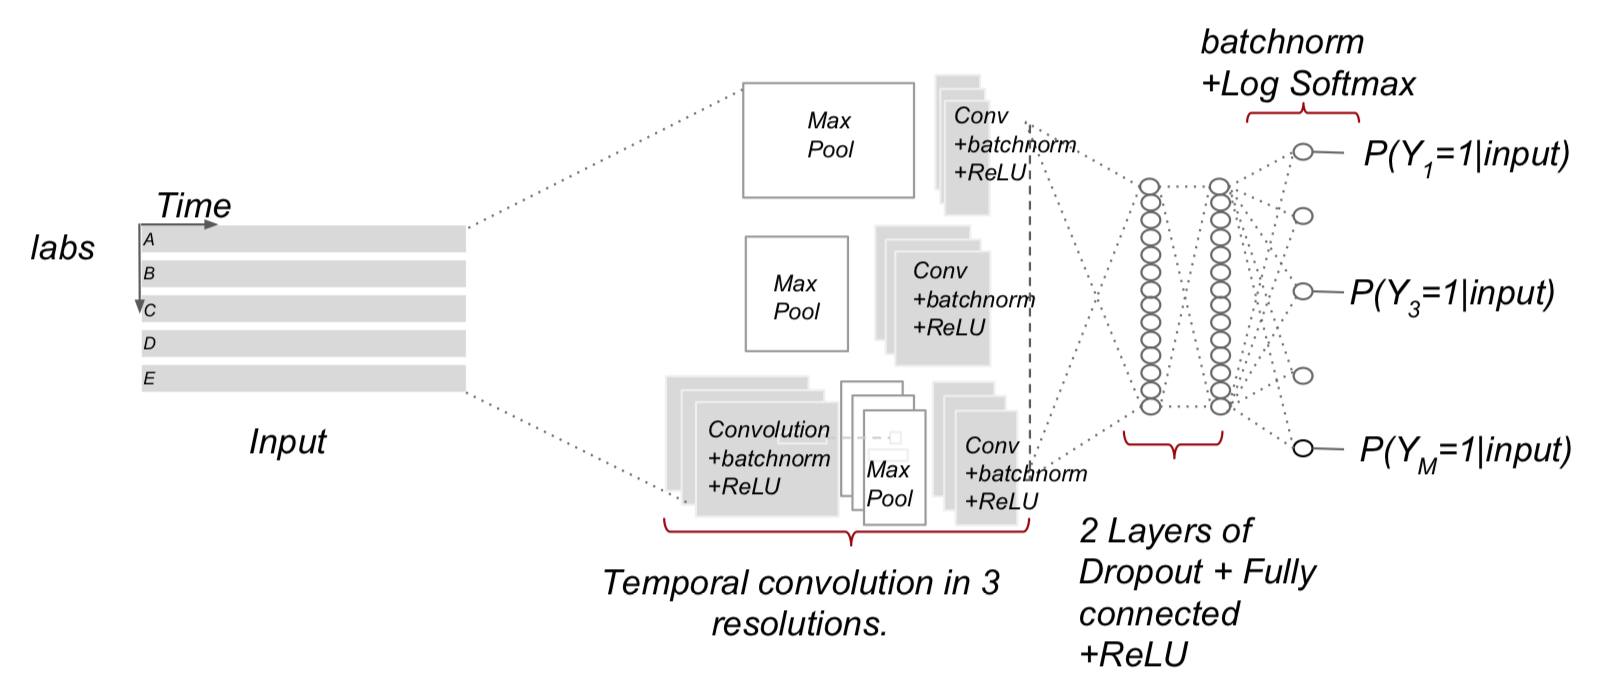
\includegraphics{covcnn.png}
\item
  Convolution across data and time according(CovNN2.R)

  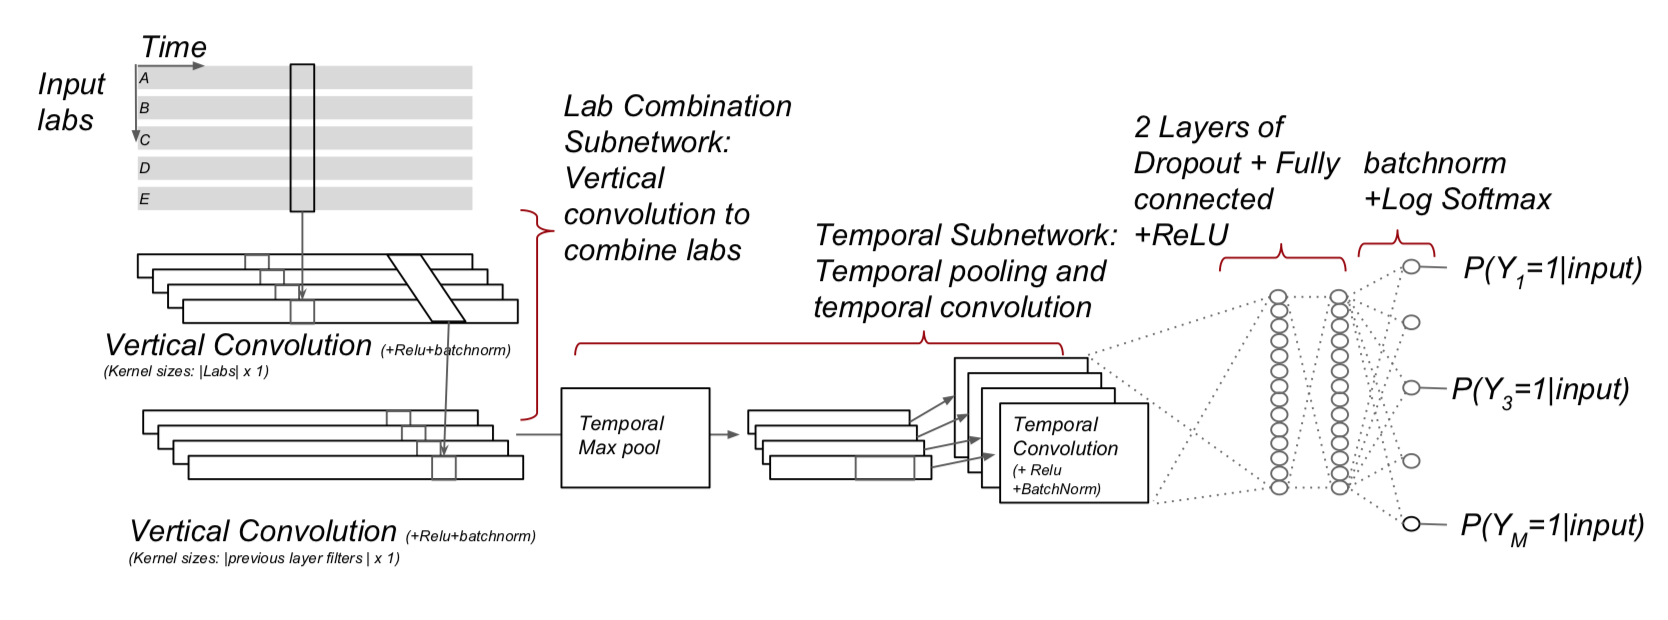
\includegraphics{covcnn2.png}

  \newpage
\end{enumerate}

Furthermore, a custom build RNN is added that uses a variational
autoencoder.

\begin{enumerate}
\def\labelenumi{\arabic{enumi}.}
\setcounter{enumi}{2}
\item
  Clinically Informing application based on Recurrent Neural Network
  (CIReNN.R)

  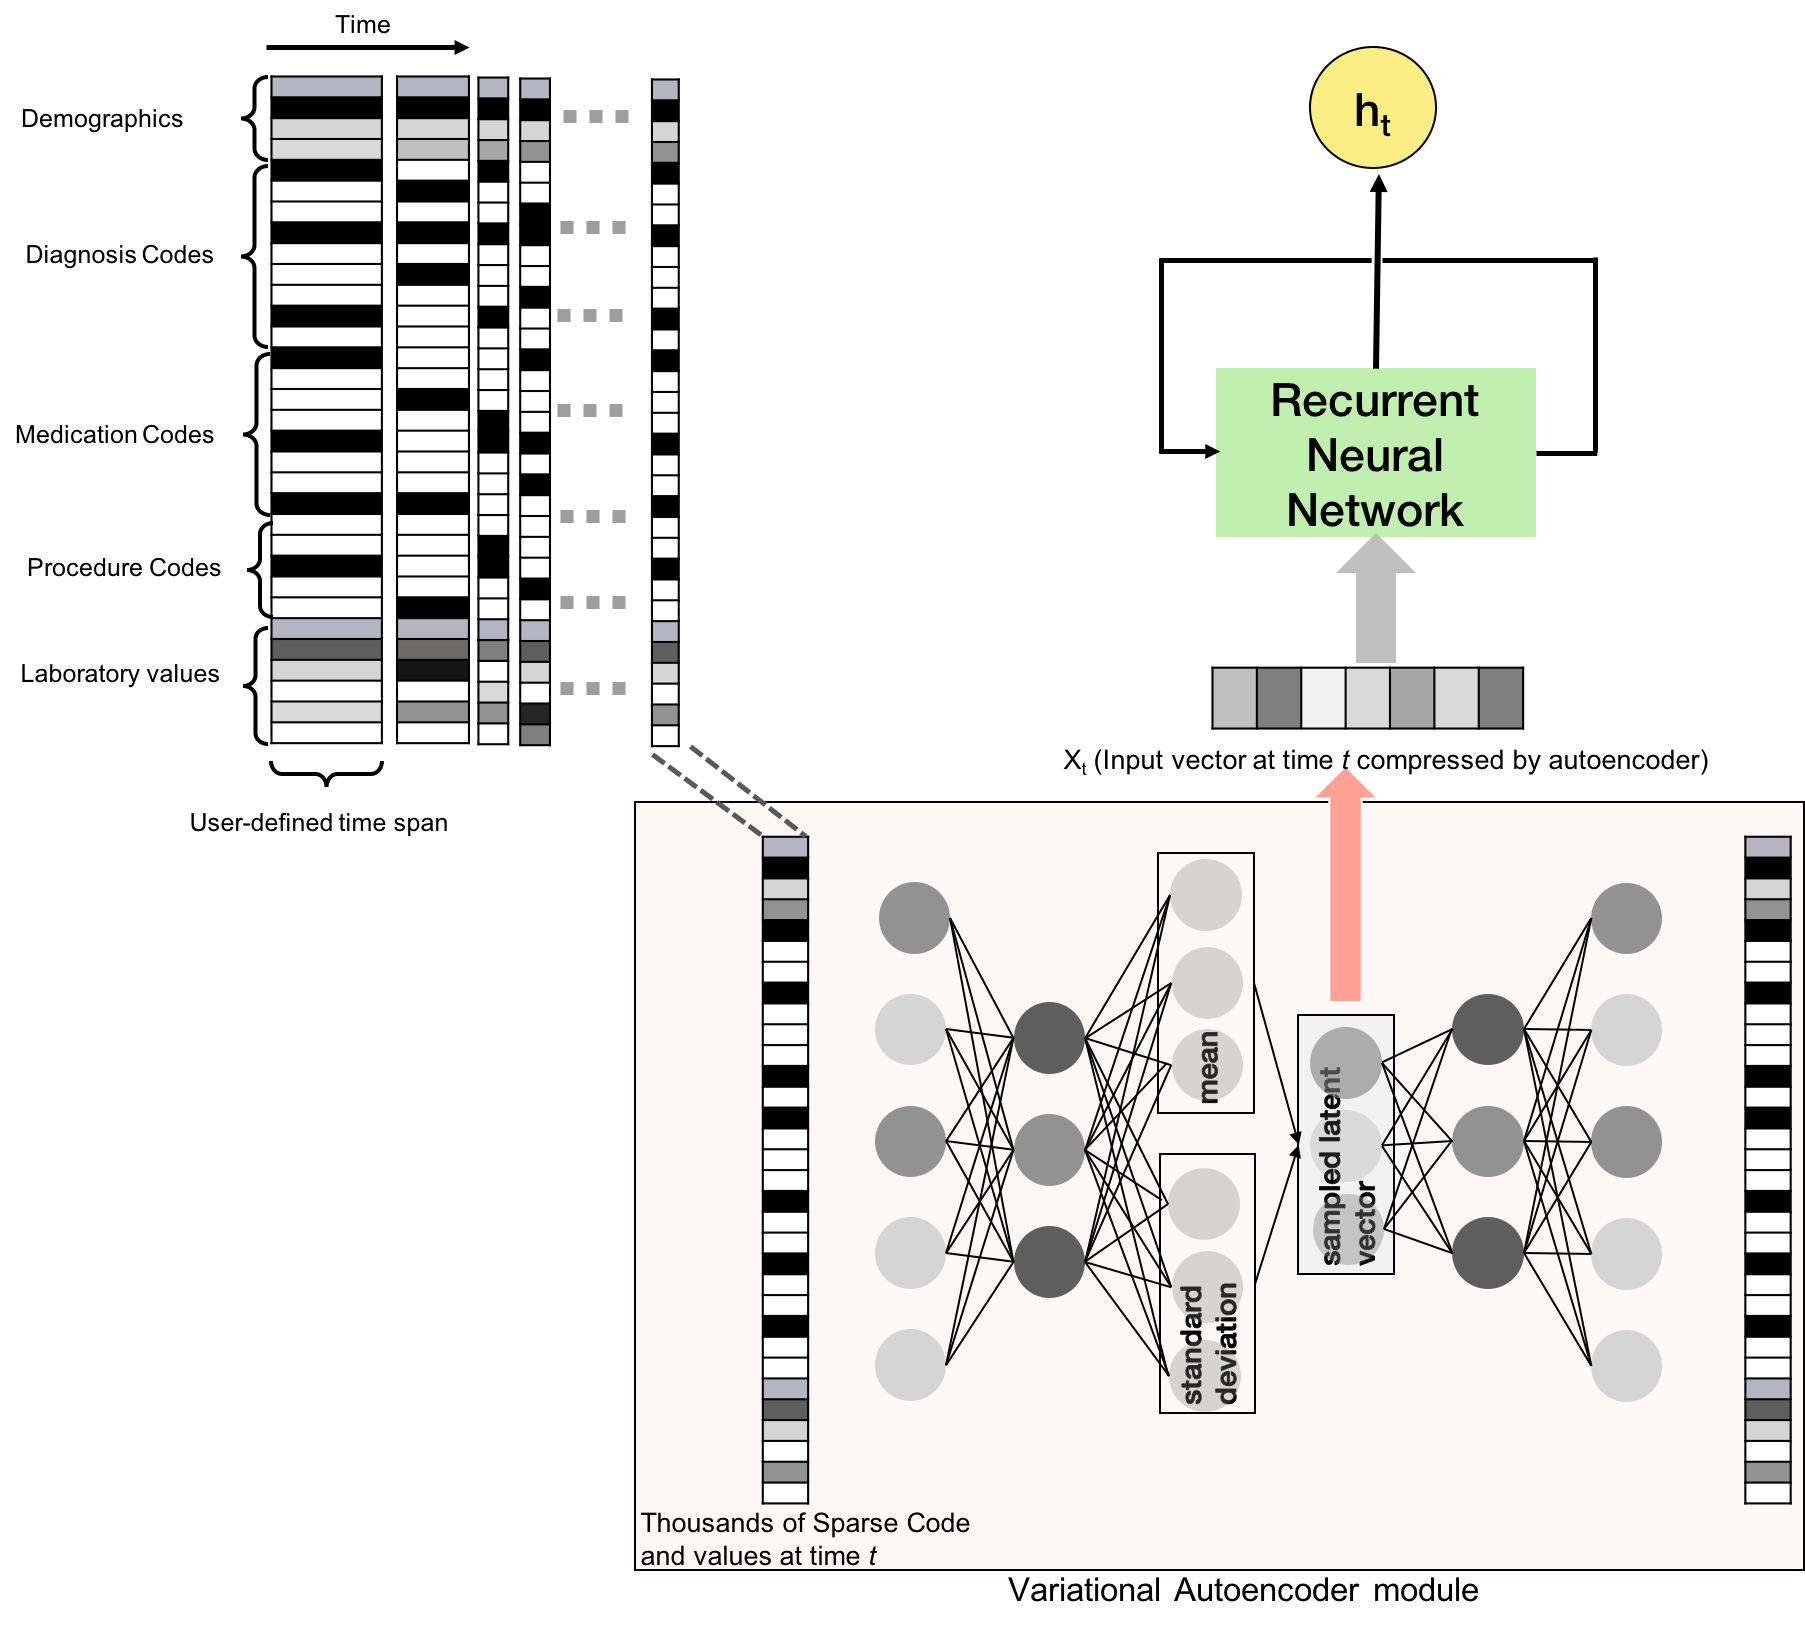
\includegraphics{cirenn.png}
\end{enumerate}

Table 2: Temporal Deep Learning Models

\begin{longtable}[]{@{}ll@{}}
\toprule
\begin{minipage}[b]{0.11\columnwidth}\raggedright
Model\strut
\end{minipage} & \begin{minipage}[b]{0.83\columnwidth}\raggedright
Hyper-parameters\strut
\end{minipage}\tabularnewline
\midrule
\endhead
\begin{minipage}[t]{0.11\columnwidth}\raggedright
CovNN\strut
\end{minipage} & \begin{minipage}[t]{0.83\columnwidth}\raggedright
batchSize (The number of samples to used in each batch during model
training), outcomeWeight (The weight assigned to the outcome), lr (The
learning rate), decay (The decay of the learning rate), dropout
({[}currently not used{]} the dropout rate for regularization), epochs
(The number of times data is used to train the model, e.g., epoches=1
means data only used once to train), filters (The number of columns
output by each convolution), kernelSize (The number of time dimensions
used for each convolution), loss (The loss function implemented), seed
(The random seed)\strut
\end{minipage}\tabularnewline
\begin{minipage}[t]{0.11\columnwidth}\raggedright
CovNN2\strut
\end{minipage} & \begin{minipage}[t]{0.83\columnwidth}\raggedright
batchSize (The number of samples to used in each batch during model
training), outcomeWeight (The weight assigned to the outcome), lr (The
learning rate), decay (The decay of the learning rate), dropout
({[}currently not used{]} the dropout rate for regularization), epochs
(The number of times data is used to train the model, e.g., epoches=1
means data only used once to train), filters (The number of columns
output by each convolution), kernelSize (The number of time dimensions
used for each convolution), loss (The loss function implemented), seed
(The random seed)\strut
\end{minipage}\tabularnewline
\begin{minipage}[t]{0.11\columnwidth}\raggedright
CIReNN\strut
\end{minipage} & \begin{minipage}[t]{0.83\columnwidth}\raggedright
units (The number of units of RNN layer - as a list of vectors),
recurrentDropout (The reccurrent dropout rate), layerDropout (The layer
dropout rate), lr (Learning rate), decay (Learning rate decay over each
update), outcomeWeight (The weight of the outcome class in the loss
function), batchSize (The number of data points to use per training
batch), epochs (Number of times to iterate over data set),
earlyStoppingMinDelta (Minimum change in the monitored quantity to
qualify as an improvement for early stopping, i.e.~an absolute change of
less than min\_delta in loss of validation data, will count as no
improvement), earlyStoppingPatience (Number of epochs with no
improvement after which training will be stopped), seed (Random seed
used by Deep Learning model)\strut
\end{minipage}\tabularnewline
\bottomrule
\end{longtable}

\hypertarget{example}{%
\subsection{Example}\label{example}}

We will now show how to use the temporal models by using CNNTorch as an
example.

You need to generate a \texttt{population} and \texttt{plpData} object
as described in more detail in
\href{https://github.com/OHDSI/PatientLevelPrediction/blob/master/inst/doc/BuildingPredictiveModels.pdf}{\texttt{BuildingPredictiveModels}
vignette}.

Note that for these algorithms you need to extracted temporal data as
described in the {[}FeatureExtraction vignette{]}
(\url{https://github.com/OHDSI/FeatureExtraction/blob/master/inst/doc/UsingFeatureExtraction.pdf})
as follows:

\begin{Shaded}
\begin{Highlighting}[]
\NormalTok{settings <-}\StringTok{ }\KeywordTok{createTemporalCovariateSettings}\NormalTok{(}\DataTypeTok{useConditionEraStart =} \OtherTok{FALSE}\NormalTok{,}
                                            \DataTypeTok{useConditionEraOverlap =} \OtherTok{FALSE}\NormalTok{,}
                                            \DataTypeTok{useConditionOccurrence =} \OtherTok{FALSE}\NormalTok{,}
                                            \DataTypeTok{useConditionEraGroupStart =} \OtherTok{FALSE}\NormalTok{,}
                                            \DataTypeTok{useConditionEraGroupOverlap =} \OtherTok{FALSE}\NormalTok{,}
                                            \DataTypeTok{useDrugExposure =} \OtherTok{FALSE}\NormalTok{,}
                                            \DataTypeTok{useDrugEraStart =} \OtherTok{FALSE}\NormalTok{,}
                                            \DataTypeTok{useDrugEraOverlap =} \OtherTok{FALSE}\NormalTok{,}
                                            \DataTypeTok{useMeasurement =} \OtherTok{FALSE}\NormalTok{,}
                                            \DataTypeTok{useMeasurementValue =} \OtherTok{TRUE}\NormalTok{,}
                                            \DataTypeTok{useMeasurementRangeGroup =} \OtherTok{FALSE}\NormalTok{,}
                                            \DataTypeTok{useProcedureOccurrence =} \OtherTok{FALSE}\NormalTok{,}
                                            \DataTypeTok{useDeviceExposure =} \OtherTok{FALSE}\NormalTok{,}
                                            \DataTypeTok{useObservation =} \OtherTok{FALSE}\NormalTok{,}
                                            \DataTypeTok{excludedCovariateConceptIds =} \KeywordTok{c}\NormalTok{(}\DecValTok{316866}\NormalTok{),}
                                            \DataTypeTok{addDescendantsToExclude =} \OtherTok{TRUE}\NormalTok{,}
                                            \DataTypeTok{temporalStartDays =} \KeywordTok{seq}\NormalTok{(}\DataTypeTok{from =} \DecValTok{-365}\NormalTok{, }
                                                                    \DataTypeTok{to =} \DecValTok{-1}\NormalTok{, }\DataTypeTok{by =} \DecValTok{12}\NormalTok{), }
                                            \DataTypeTok{temporalEndDays =} \KeywordTok{c}\NormalTok{(}\KeywordTok{seq}\NormalTok{(}\DataTypeTok{from =} \DecValTok{-353}\NormalTok{, }
                                                                    \DataTypeTok{to =} \DecValTok{0}\NormalTok{, }\DataTypeTok{by =} \DecValTok{12}\NormalTok{), }\DecValTok{0}\NormalTok{))}

\NormalTok{plpData <-}\StringTok{ }\KeywordTok{getPlpData}\NormalTok{(}\DataTypeTok{connectionDetails =}\NormalTok{ connectionDetails,}
                        \DataTypeTok{cdmDatabaseSchema =}\NormalTok{ cdmDatabaseSchema,}
                        \DataTypeTok{cohortDatabaseSchema =} \StringTok{"results"}\NormalTok{,}
                        \DataTypeTok{cohortTable =} \StringTok{"cohort"}\NormalTok{,}
                        \DataTypeTok{cohortId =} \DecValTok{11}\NormalTok{,}
                        \DataTypeTok{covariateSettings =}\NormalTok{ settings,}
                        \DataTypeTok{outcomeDatabaseSchema =}\NormalTok{ resultsDatabaseSchema,}
                        \DataTypeTok{outcomeTable =} \StringTok{"cohort"}\NormalTok{,}
                        \DataTypeTok{outcomeIds =} \DecValTok{25}\NormalTok{,}
                        \DataTypeTok{cdmVersion =} \DecValTok{5}\NormalTok{)}
\end{Highlighting}
\end{Shaded}

Each CNN/RNN has several hyper-parameters that can be set as shown in
the Tables above, but for this example we take the defaults.

\begin{Shaded}
\begin{Highlighting}[]
\CommentTok{# specify the the CNN}
\NormalTok{model <-}\StringTok{ }\KeywordTok{setCNNTorch}\NormalTok{(}\DataTypeTok{cnn_type=}\StringTok{'CNN'}\NormalTok{)}
\end{Highlighting}
\end{Shaded}

Run the model training, for example with a testFraction = 0.2 and a
split by person:

\begin{Shaded}
\begin{Highlighting}[]
\NormalTok{results <-}\StringTok{ }\NormalTok{PatientLevelPrediction}\OperatorTok{::}\KeywordTok{runPlp}\NormalTok{(population, plpData, model,}
                                          \DataTypeTok{testSplit=}\StringTok{'person'}\NormalTok{,}
                                          \DataTypeTok{testFraction=}\FloatTok{0.2}\NormalTok{,}
                                          \DataTypeTok{nfold=}\DecValTok{3}\NormalTok{, }
                                          \DataTypeTok{splitSeed=}\DecValTok{1000}\NormalTok{) }
\end{Highlighting}
\end{Shaded}

\hypertarget{apply-the-trained-deep-learning-model}{%
\section{Apply the trained Deep Learning
model}\label{apply-the-trained-deep-learning-model}}

Applying a Deep Learning is identical to the other models in the
package:

\begin{Shaded}
\begin{Highlighting}[]
\CommentTok{# load the trained model}
\NormalTok{plpModel <-}\StringTok{ }\KeywordTok{loadPlpModel}\NormalTok{(}\KeywordTok{getwd}\NormalTok{(), }\StringTok{"<your model>"}\NormalTok{)}

\CommentTok{# load the new plpData (should have the same temporal features!) and create the population}
\NormalTok{plpData <-}\StringTok{ }\KeywordTok{loadPlpData}\NormalTok{(}\KeywordTok{getwd}\NormalTok{(), }\StringTok{"<your data>"}\NormalTok{)}

\NormalTok{populationSettings <-}\StringTok{ }\NormalTok{plpModel}\OperatorTok{$}\NormalTok{populationSettings}
\NormalTok{populationSettings}\OperatorTok{$}\NormalTok{plpData <-}\StringTok{ }\NormalTok{plpData}
\NormalTok{population <-}\StringTok{ }\KeywordTok{do.call}\NormalTok{(createStudyPopulation, populationSettings)  }

\CommentTok{# apply the trained model on the new data}
\NormalTok{validationResults <-}\StringTok{ }\KeywordTok{applyModel}\NormalTok{(population, plpData, plpModel)}
\end{Highlighting}
\end{Shaded}

\hypertarget{adding-new-architectures}{%
\section{Adding new architectures}\label{adding-new-architectures}}

It is possible to add new architectures in our framework using PyTorch
or R Keras. We are happy to help you with this, please post your
questions on the
\href{www.github.com/OHDSI/PatientLevelPrediction/issues}{issue tracker}
of the package.

\hypertarget{acknowledgments}{%
\section{Acknowledgments}\label{acknowledgments}}

Considerable work has been dedicated to provide the
\texttt{PatientLevelPrediction} package.

\begin{Shaded}
\begin{Highlighting}[]
\KeywordTok{citation}\NormalTok{(}\StringTok{"PatientLevelPrediction"}\NormalTok{)}
\end{Highlighting}
\end{Shaded}

\begin{verbatim}
## 
## To cite PatientLevelPrediction in publications use:
## 
## Reps JM, Schuemie MJ, Suchard MA, Ryan PB, Rijnbeek P (2018). "Design and
## implementation of a standardized framework to generate and evaluate patient-level
## prediction models using observational healthcare data." _Journal of the American
## Medical Informatics Association_, *25*(8), 969-975. <URL:
## https://doi.org/10.1093/jamia/ocy032>.
## 
## A BibTeX entry for LaTeX users is
## 
##   @Article{,
##     author = {J. M. Reps and M. J. Schuemie and M. A. Suchard and P. B. Ryan and P. Rijnbeek},
##     title = {Design and implementation of a standardized framework to generate and evaluate patient-level prediction models using observational healthcare data},
##     journal = {Journal of the American Medical Informatics Association},
##     volume = {25},
##     number = {8},
##     pages = {969-975},
##     year = {2018},
##     url = {https://doi.org/10.1093/jamia/ocy032},
##   }
\end{verbatim}

\textbf{Please reference this paper if you use the PLP Package in your
work:}

\href{http://dx.doi.org/10.1093/jamia/ocy032}{Reps JM, Schuemie MJ,
Suchard MA, Ryan PB, Rijnbeek PR. Design and implementation of a
standardized framework to generate and evaluate patient-level prediction
models using observational healthcare data. J Am Med Inform Assoc.
2018;25(8):969-975.}

\end{document}
